\documentclass[18pt]{beamer}
\usepackage{templates/beamerthemekit}
\usepackage[export]{adjustbox}
\usepackage{tikz}
\usepackage{url}
\usepackage{amsmath}
\usepackage{marvosym} % \MVRIGHTarrow
\usepackage{stmaryrd} % \shortrightarrow
\usepackage{textcomp} % \textrightarrow
\usepackage{svg}

\title[Project discussion]{Towards Bringing Together Numerical Methods for Partial Differential Equation and Deep Neural Networks}
\subtitle{Project discussion, Supervisor - Markus Hoffmann}
\author{Stanislav Arnaudov}
\institute{Chair for Computer Architecture and Parallel Processing}
\date{September 26, 2019}
\selectlanguage{english}

% \usepackage[style=verbose,backend=bibtex]{biblatex}
% \bibliography{bib}
% \bibliographystyle{plain}

\newcommand{\semitransp}[2][35]{\color{fg!#1}#2 \color{fg}}

\begin{document}

\begin{frame}
 \titlepage
\end{frame}

\section{Motivation}

\begin{frame}
  \frametitle{Problem definition and motivation}
  \begin{columns}
    \begin{column}{0.5\textwidth}
      Partial differential equation (PDEs)
      \begin{itemize}
      \item used in simulations
      \item hard to solve numerically
      \item solutions have image representation
      \end{itemize}
      \vspace{0.25cm}
      \textbf{Idea}: study non-classical ways for generating solutions of PDEs
      \vspace{-0.5cm}
    \end{column}
    \begin{column}{0.5\textwidth}
      \begin{center}
        \begin{figure}[htb]
          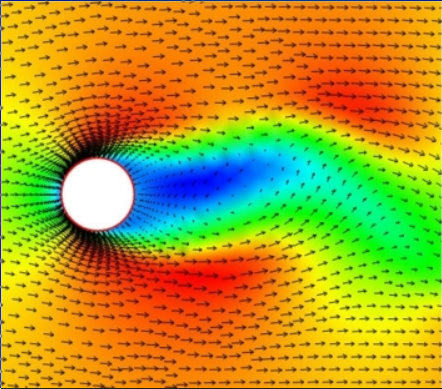
\includegraphics[scale=0.35]{images/pde}
          \caption{Flow Simulation\footnotemark}
        \end{figure}
      \end{center}
    \end{column}
    \footnotetext{``Team for Advanced Flow Simulation and Modeling'', Professor Tayfun E. Tezduyar, Sunil Sathe}
  \end{columns}
\end{frame}

\begin{frame}
  \frametitle{Problem definition and motivation}
  Deep neural networks (DNNs)
  \begin{itemize}
  \item hot topic in recent years
  \item impressive results in image processing tasks
  \end{itemize}
  \textbf{Idea}: Use DNNs in order to solve PDEs \\
  \pause
  \vspace{1cm}
  \textbf{Research topic}: The applicability of DNNs in generating solutions for PDEs.
\end{frame}



\begin{frame}[t]
  \frametitle{Problem definition and motivation}
  Concrete problem to study
\end{frame}


\begin{frame}[t]
  \frametitle{Problem definition and motivation}
  Concrete problem to study
  \vspace*{0.3cm}
  \begin{center}
    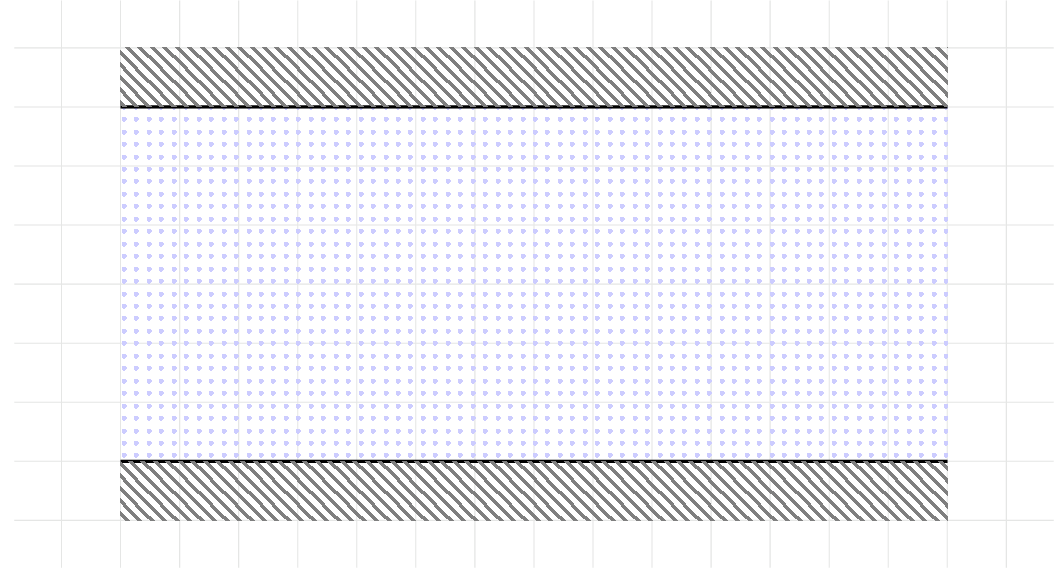
\includegraphics[scale=0.2]{images/channel/flow_0}
  \end{center}
  A channel with \textit{incompressible} fluid in it.
\end{frame}


\begin{frame}[t]
  \frametitle{Problem definition and motivation}
  Concrete problem to study
  \vspace*{0.3cm}
  \begin{center}
    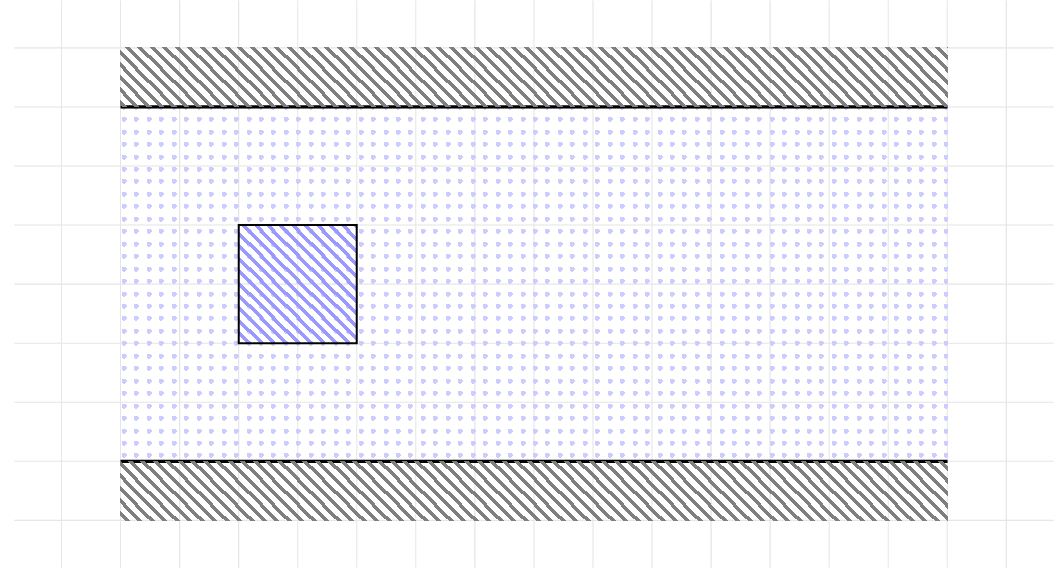
\includegraphics[scale=0.2]{images/channel/flow_1}
  \end{center}
  An object placed inside of the channel.
\end{frame}


\begin{frame}[t]
  \frametitle{Problem definition and motivation}
  Concrete problem to study
  \vspace*{0.3cm}
  \begin{center}
    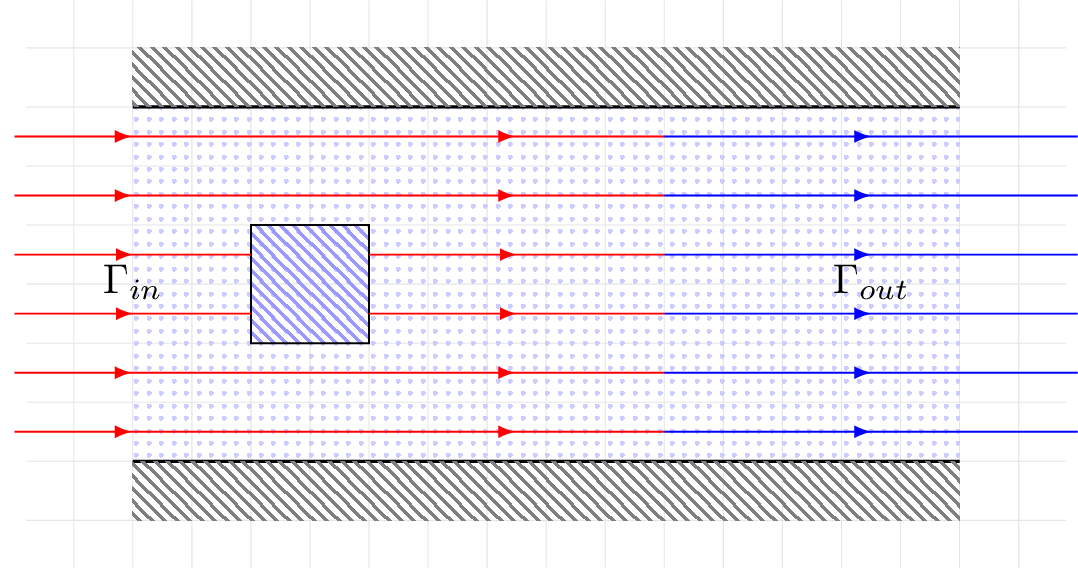
\includegraphics[scale=0.2]{images/channel/flow_2}
  \end{center}
  The fluid is flowing in from the one side and flowing out from the other one.
\end{frame}


\begin{frame}[t]
  \frametitle{Problem definition and motivation}
  % \begin{columns}
  %   \begin{column}{0.5\textwidth}
  %     \begin{center}
  %       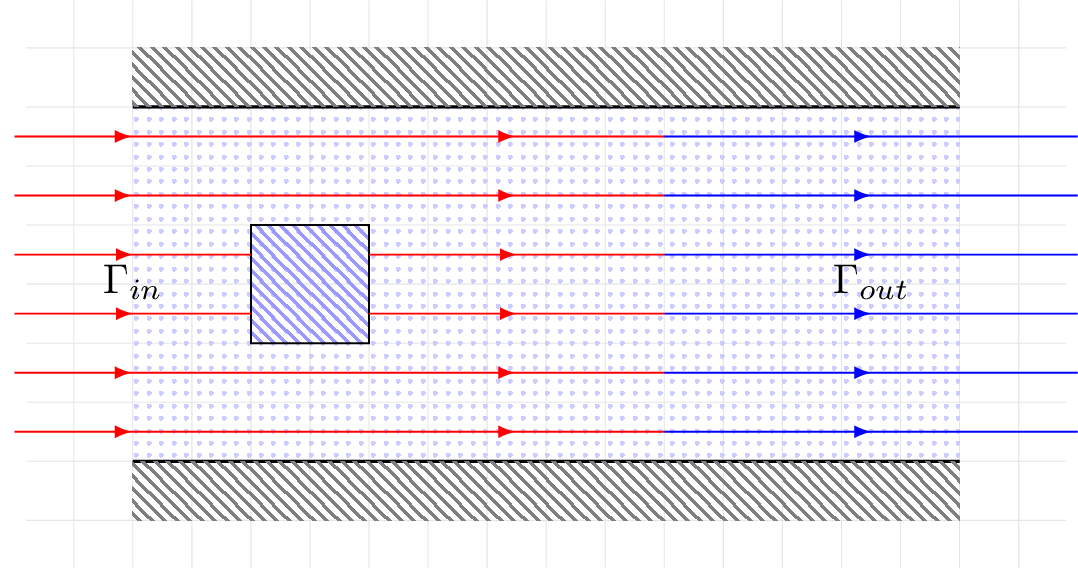
\includegraphics[scale=0.13]{images/channel/flow_2}
  %     \end{center}
  %   \end{column}
  %   \begin{column}{0.5\textwidth}
  %   \end{column}
  % \end{columns}
  \begin{block}{Incompressible Navier-Stokes Equation}
  \begin{align*}
          -\nu\Delta u + (u\cdot\nabla)u + \frac{1}{\rho}\nabla p =& 0,  \quad\text{in}\: \Omega\\
          \nabla\cdot u =& 0, \quad\text{in}\: \Omega \\
          u =& g, \quad\text{on}\: \Gamma_{in} \\
          (-\mathcal{I}p + \nu\nabla u)\cdot n =& 0, \quad\text{on}\: \Gamma_{out} \\
          u =& 0, \quad\text{on}\:  \partial\Omega\slash (\overline{\Gamma_{in}\cup\Gamma_{out}})
  \end{align*}
  \end{block}
  \vspace*{1.5cm}
\end{frame}

\begin{frame}[t]
  \frametitle{Problem definition and motivation}
  \vspace*{-0.5cm}
  \begin{block}{Incompressible Navier-Stokes Equation}
  \begin{align*}
           -\nu\Delta u + (u\cdot\nabla)u + \frac{1}{\tikz[baseline]{
            \node[fill=blue!20,anchor=base] (t1)
            {$\rho$};}}\nabla p =& 0,  \quad\text{in}\: \Omega\\
          \nabla\cdot u =& 0, \quad\text{in}\: \Omega \\
          u =& \tikz[baseline]{
            \node[fill=blue!20,anchor=base] (t1)
            {$g$};}, \quad\text{on}\: \Gamma_{in} \\
          (-\mathcal{I}p + \nu\nabla u)\cdot \tikz[baseline]{
            \node[fill=blue!20,anchor=base] (t1)
            {$n$};} =& 0, \quad\text{on}\: \Gamma_{out} \\
          u =& 0, \quad\text{on}\:  \partial\Omega\slash (\overline{\Gamma_{in}\cup\Gamma_{out}})
  \end{align*}
\end{block}
Parameters:
\begin{itemize}
\item fluid viscosity and density -- $\rho$ and $n$
\item inflow speed -- $g$
\end{itemize}
\end{frame}

\begin{frame}[t]
  \frametitle{Problem definition and motivation}
  \vspace*{-0.5cm}
  \begin{block}{Incompressible Navier-Stokes Equation}
    \begin{align*}
      -\nu\Delta \tikz[baseline]{
            \node[fill=red!20,anchor=base] (t1)
            {$u$};} + (\tikz[baseline]{
            \node[fill=red!20,anchor=base] (t1)
            {$u$};}\cdot\nabla)\tikz[baseline]{
            \node[fill=red!20,anchor=base] (t1)
            {$u$};} + \frac{1}{\rho}\nabla \tikz[baseline]{
            \node[fill=red!20,anchor=base] (t1)
            {$p$};} =& 0,  \quad\text{in}\: \Omega\\
      \nabla\cdot \tikz[baseline]{
            \node[fill=red!20,anchor=base] (t1)
            {$u$};} =& 0, \quad\text{in}\: \Omega \\
      \tikz[baseline]{
            \node[fill=red!20,anchor=base] (t1)
            {$u$};} =& g, \quad\text{on}\: \Gamma_{in} \\
      (-\mathcal{I}\tikz[baseline]{
            \node[fill=red!20,anchor=base] (t1)
            {$p$};} + \nu\nabla \tikz[baseline]{
            \node[fill=red!20,anchor=base] (t1)
            {$u$};})\cdot n =& 0, \quad\text{on}\: \Gamma_{out} \\
      \tikz[baseline]{
            \node[fill=red!20,anchor=base] (t1)
            {$u$};} =& 0, \quad\text{on}\:  \partial\Omega\slash (\overline{\Gamma_{in}\cup\Gamma_{out}})
  \end{align*}
\end{block}
Solutions:
\begin{itemize}
\item velocity field -- $u$
\item pressure field -- $p$
\end{itemize}
\end{frame}


\begin{frame}[t]
  \frametitle{Problem definition and motivation}
  DNNs in the context of the described problem
  \begin{itemize}
  \item The solutions of the PDE can be visualized as images
  \item DNNs perform well on image processing tasks
  \end{itemize}
  \pause
  $\Longrightarrow$ use DNNs to generate solutions of the simulation in image form \\
\end{frame}

\begin{frame}[t]
  \frametitle{Problem definition and motivation}
  DNNs in the context of the described problem
  \begin{itemize}
  \item The solutions of the PDE can be visualized as images
  \item DNNs perform well on image processing tasks
  \end{itemize}
  $\Longrightarrow$ use DNNs to generate solutions of the simulation in image form \\
  \begin{center}
    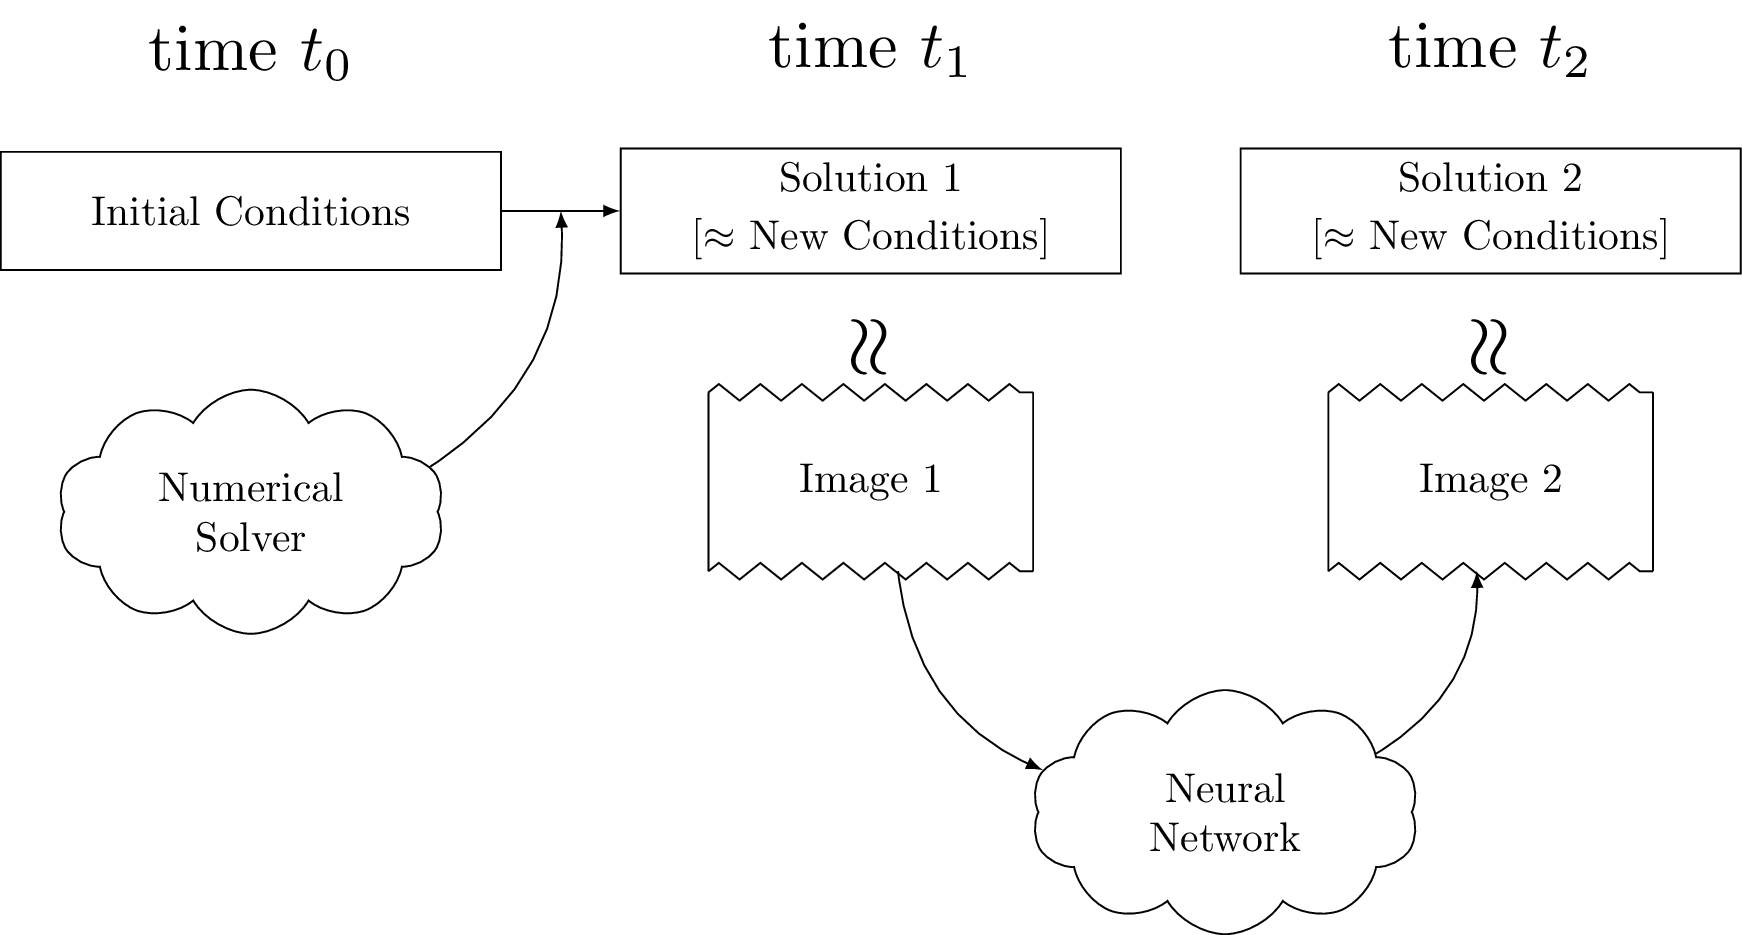
\includegraphics[scale=0.16]{images/new/overview}
  \end{center}
\end{frame}


\begin{frame}[t]
  \frametitle{Problem definition and motivation}
  DNNs in the context of the described problem
  \begin{itemize}
  \item The solutions of the PDE can be visualized as images
  \end{itemize}
  $\Longrightarrow$ use DNNs to generate solutions of the simulation in image form \\
  \vspace*{1.5cm}
  \begin{itemize}
  \item Why use images as input for the network?
  \item Why are images useful as network output?
  \end{itemize}
\end{frame}

\begin{frame}
  \frametitle{Problem definition and motivation}
  Images of simulations
    \begin{columns}
      \begin{column}{0.5\textwidth}
        \begin{center}
          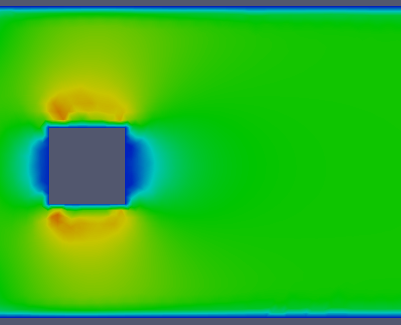
\includegraphics[scale=0.3]{images/flow-1}
          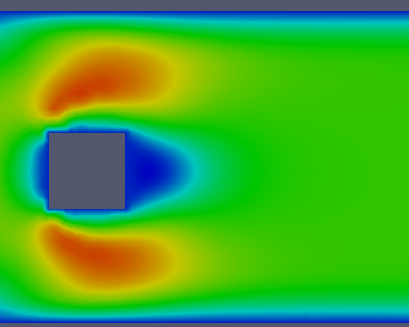
\includegraphics[scale=0.3]{images/flow-3}
        \end{center}
      \end{column}
      \hspace*{-1.5cm}
    \begin{column}{0.5\textwidth}
      \begin{center}
        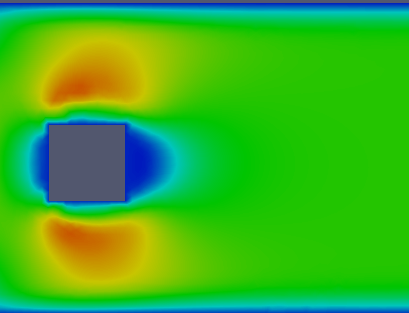
\includegraphics[scale=0.3]{images/flow-2}
        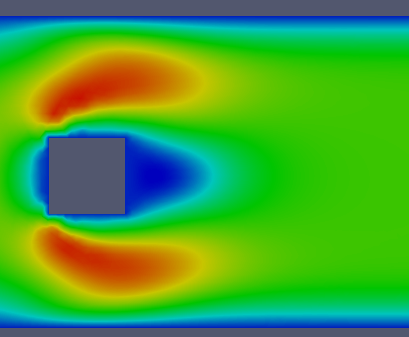
\includegraphics[scale=0.3]{images/flow-4}
      \end{center}
    \end{column}
  \end{columns}
\end{frame}


\section{Research Definition}
\begin{frame}[t]
  \frametitle{Definition}
  \begin{block}{Research topic}
    The applicability of DNNs in generating solutions for PDEs in numerical simulation context.
  \end{block}
  \begin{block}{Research question}
    To what extend can DNNs generalize the parameters of a simulation of an incompressible fluid flow inside a channel according to the Navier-Stokes equation? The parameters of interest are:
    \begin{itemize}
    \item Fluid viscosity and density
    \item Inflow speed
    \end{itemize}
    To be studied is a DNN-based model that processes the image representations of the solutions of the simulation.
  \end{block}
\end{frame}


\section{Related Work}
\begin{frame}[t]
  \frametitle{Related Work \& State-of-the-Art}
  \begin{columns}[t]
    \begin{column}{0.5\textwidth}
    \end{column}
    \begin{column}{0.5\textwidth}
    \end{column}
  \end{columns}
\end{frame}


\begin{frame}[t]
  \frametitle{Related Work \& State-of-the-Art}
  DNNs in Image processing\\
  {\footnotesize (with focus on image-to-image mapping)}
  \begin{itemize}
  \item Used in wide variety of tasks
    \begin{itemize}
    \item Image Segmentation
    \item Semantic Image Synthesis
    \end{itemize}
  \item We build upon the work of \textit{pix2pixHD}\footnotemark
    \begin{itemize}
    \item ``general-purpose solution to image-to-image translation problems''
    \item has not yet been applied to generation of simulation images
    \end{itemize}
  \end{itemize}
  \footnotetext{Ting-Chun Wang, Ming-Yu Liu, Jun-Yan Zhu, Andrew Tao, Jan Kautz, and Bryan Catanzaro. ``High-resolution image synthesis and semantic manipulation with conditional gans.''}
\end{frame}


\begin{frame}[t]
  \frametitle{Related Work \& State-of-the-Art}  
  Neural Networks in numerical simulations\\
  {\footnotesize (with focus on Navier-Stoke problems)}
  \begin{itemize}

  \item Hidden Fluid Mechanics: A Navier-Stokes Informed Deep Learning Framework for Assimilating Flow Visualization Data\footnotemark
    \begin{itemize}
    \item tailored DNN-model
    \item maps concentration of substance (in time and space) to velocity and pressure
    \end{itemize}
    
    \item Study of Deep Learning Methods for Reynolds-Averaged Navier-Stokes Simulations of Airfoil Flows\footnotemark
    \begin{itemize}
    \item considers the Reynolds-Averaged Navier-Stokes equation
    \item maps boundary conditions to velocity and pressure fields
      % \item does not test with different geometries and fluid-parameters 
    \end{itemize}
    
  \end{itemize}
  \footnotetext[3]{Maziar Raissi and Alireza Yazdani and George Em Karniadakis. (2018) ``....'' 1808.04327}
  \footnotetext{Nils Thuerey, Konstantin Weissenow, Harshit Mehrotra, Nischal Mainali, Lukas Prantl. (2018). ``....''. 481-490. 1810.08217. }
\end{frame}



\section{Methodology}
\begin{frame}[t]
  \frametitle{Methodology}
\end{frame}


\begin{frame}[t]
  \frametitle{Methodology}
  Standard machine learning project\\
\end{frame}

\begin{frame}[t]
  \frametitle{Methodology}
  Standard machine learning project.\\
  $\Longrightarrow$
  \begin{itemize}
  \item[1)] Generate training data
  \item[2)] Build and train model
  \item[3)] Evaluate model
  \end{itemize}
\end{frame}

\begin{frame}[t]
  \frametitle{Methodology}
  \begin{columns}[t]
    \begin{column}{0.4\textwidth}
      \begin{itemize}
      \item[1)] Generate training data
      \item[2)] \semitransp{Build and train model}
      \item[3)] \semitransp{Evaluate model}
      \end{itemize}
    \end{column}
    \begin{column}{0.6\textwidth}
      \begin{itemize}
      \item Use \textit{HiFlow} to run simulations
      \item Use \textit{ParaView} to generate images based on the simulation results
      \end{itemize}
    \end{column}
  \end{columns}
\end{frame}


\begin{frame}[t]
  \frametitle{Methodology}
  \begin{columns}[t]
    \begin{column}{0.4\textwidth}
      \begin{itemize}
      \item[1)] \semitransp{Generate training data}
      \item[2)] Build and train model
      \item[3)] \semitransp{Evaluate model}
      \end{itemize}
    \end{column}
    \begin{column}{0.6\textwidth}
      \begin{itemize}
      \item Implement a model in \textit{PyTorch}
        \begin{itemize}
          \item following the framework of \textit{pix2pix}
          \item \textit{GAN} (Generative Adversarial Network) based approach
          \end{itemize}
          \item Train with the generated data
      \end{itemize}
    \end{column}
  \end{columns}

\end{frame}


\begin{frame}[t]
  \frametitle{Methodology}
  \begin{columns}[t]
    \begin{column}{0.4\textwidth}
      \begin{itemize}
      \item[1)] \semitransp{Generate training data}
      \item[2)] \semitransp{Build and train model}
      \item[3)] Evaluate model
      \end{itemize}
    \end{column}
    \begin{column}{0.6\textwidth}
      \begin{itemize}
      \item Deviation from the true solution-image as an error measurement
      \item Two evaluation cases to consider:
        \begin{itemize}
        \item Error when applying the model on individual data points
        \item Error when applying the model recursively
        \end{itemize}
      \end{itemize}      
    \end{column}
  \end{columns}
\end{frame}


\begin{frame}[t]
  \frametitle{Methodology}
  \vspace{-1cm}
  \begin{columns}[t]
    \begin{column}{0.5\textwidth}
      \begin{center}
        {\large \underline{Individual Images}}
        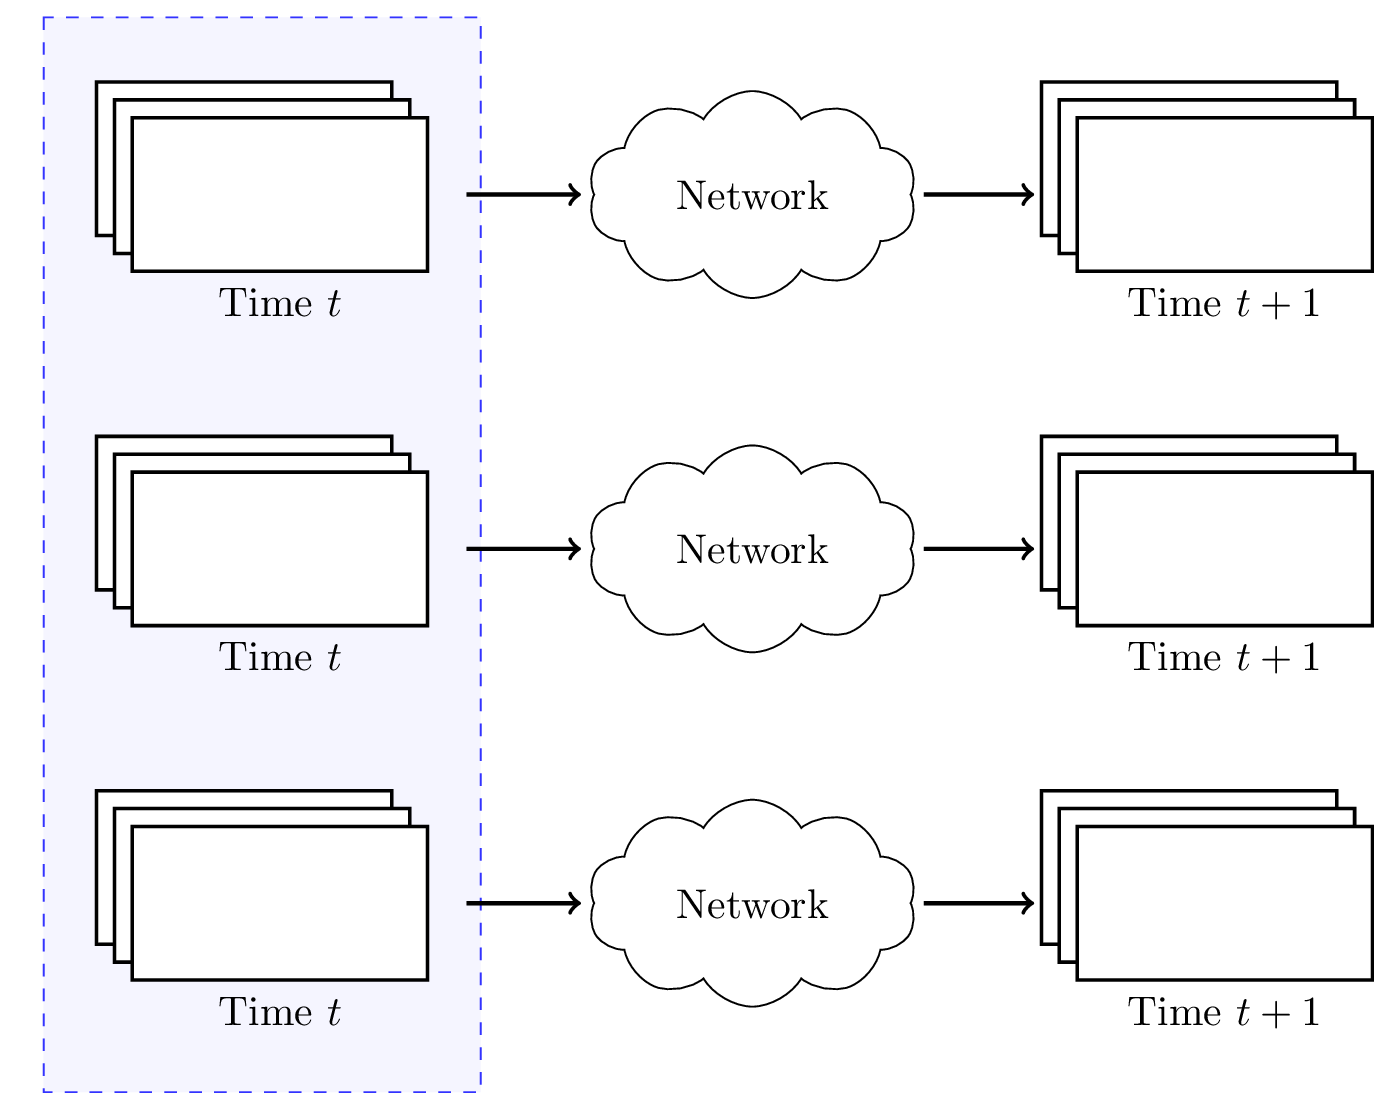
\includegraphics[scale=0.12]{images/simple_eval}
      \end{center}
    \end{column}
    \begin{column}{0.5\textwidth}
      \begin{center}
        {\large \underline{Recursive Application}}
        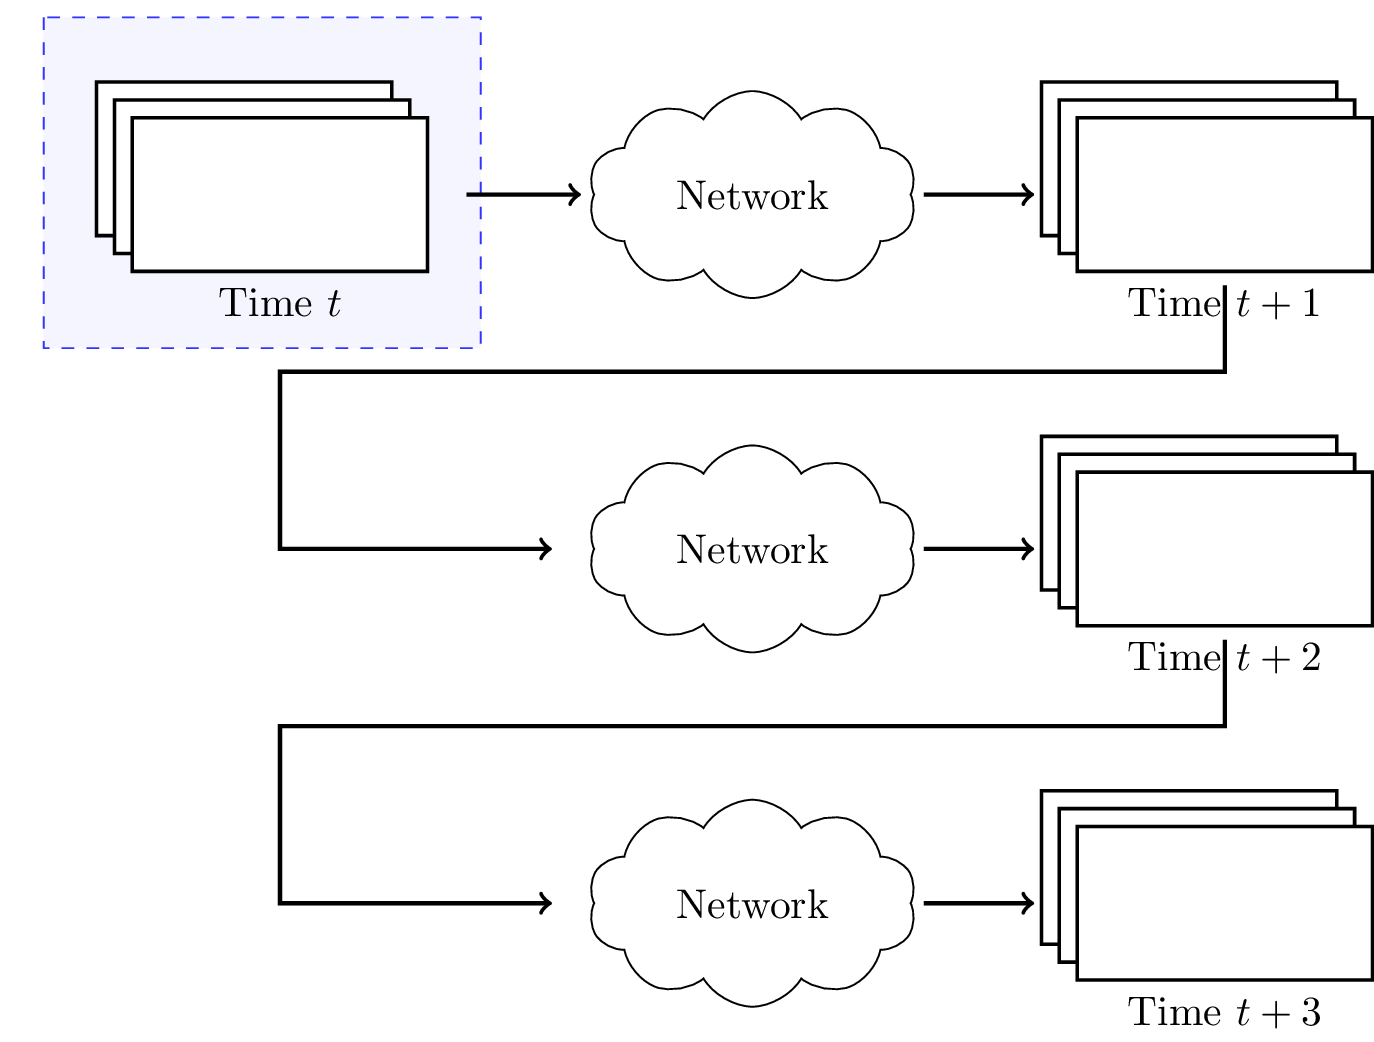
\includegraphics[scale=0.12]{images/rec_eval}
      \end{center}
    \end{column}
  \end{columns}
\end{frame}


\begin{frame}[t]
  \frametitle{Definition}
  ...
  \begin{block}{Research question}
    To what extend can DNNs generalize the parameters of a simulation of an incompressible fluid flow inside a channel according to the Navier-Stoke equation? The parameters of interest are:
    \tikz[baseline]{
      \node[fill=red!20, anchor=base]
      {
        \begin{minipage}{5cm}
        \begin{itemize}
        \item Fluid viscosity and density
        \item Inflow speed
        \end{itemize}
        \end{minipage}
      };
    }\\
    To be studied is a DNN-based model that processes the image representations of the solutions of the simulation.
  \end{block}
  \pause
  $\Longrightarrow$ \textbf{Goal:} Build a separate model for each of the cases.
\end{frame}


\section{Workplan}
\begin{frame}[t]
  \frametitle{Methodology\textbackslash Workplan}
  \begin{columns}[t]
    \begin{column}{0.35\textwidth}
      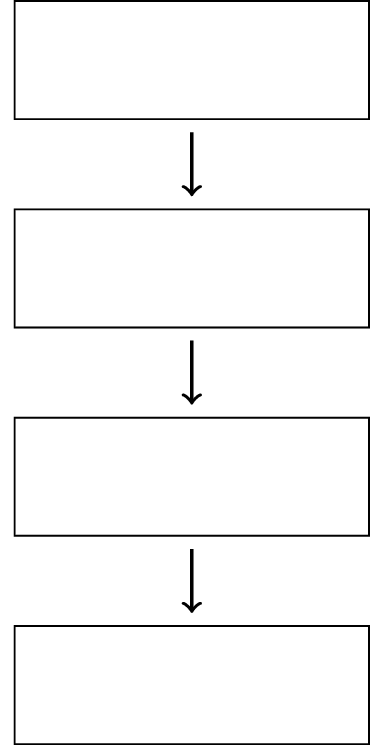
\includegraphics[scale=0.25]{images/meth/meth_1}
    \end{column}
    \begin{column}[t]{0.65\textwidth}
      \vspace*{-7cm}
    \end{column}
  \end{columns}
\end{frame}


\begin{frame}[t]
  \frametitle{Methodology\textbackslash Workplan}
  \begin{columns}[t]
    \begin{column}{0.35\textwidth}
      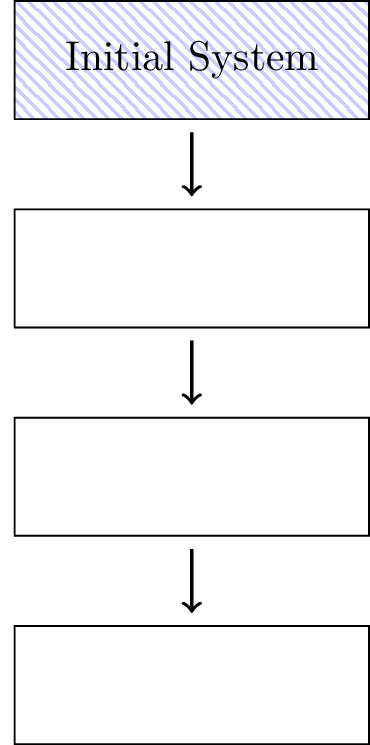
\includegraphics[scale=0.25]{images/meth/meth_2}
    \end{column}
    \begin{column}[t]{0.65\textwidth}
      \vspace*{-5cm}
      \begin{itemize}
      \item Data generation
      \item Implementation of core components
        \begin{itemize}
        \item Data loader
        \item Model architecture
        \item Training infrastructure
        \item Evaluation infrastructure
        \end{itemize}
      \item Training and evaluating a baseline model
        \begin{itemize}
        \item works \underline{only} with image data
        \item thought of as the basis for further development
        \end{itemize}
      \end{itemize}
    \end{column}
  \end{columns}
\end{frame}


\begin{frame}[t]
  \frametitle{Methodology\textbackslash Workplan}
  \begin{columns}[t]
    \begin{column}{0.35\textwidth}
      \includegraphics[scale=0.25]{images/meth/meth_3}
    \end{column}
    \begin{column}[t]{0.65\textwidth}
      \vspace*{-5cm}
      \begin{itemize}
      \item Model modifications
        \begin{itemize}
        \item fluid viscosity and density as input
        \end{itemize}
      \item Training and evaluating
      \end{itemize}
    \end{column}
  \end{columns}
\end{frame}


\begin{frame}[t]
  \frametitle{Methodology\textbackslash Workplan}
  \begin{columns}[t]
    \begin{column}{0.35\textwidth}
      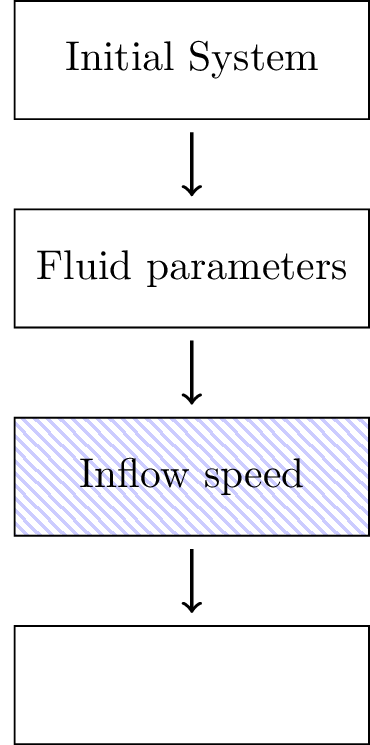
\includegraphics[scale=0.25]{images/meth/meth_4}
    \end{column}
    \begin{column}[t]{0.65\textwidth}
      \vspace*{-5cm}
      \begin{itemize}
      \item Model modifications
        \begin{itemize}
        \item inflow speed as input
        \end{itemize}
      \item Training and evaluating
      \end{itemize}
    \end{column}
  \end{columns}
\end{frame}


\begin{frame}
  \frametitle{Methodology\textbackslash Workplan}
  \begin{columns}
    \begin{column}{0.35\textwidth}
      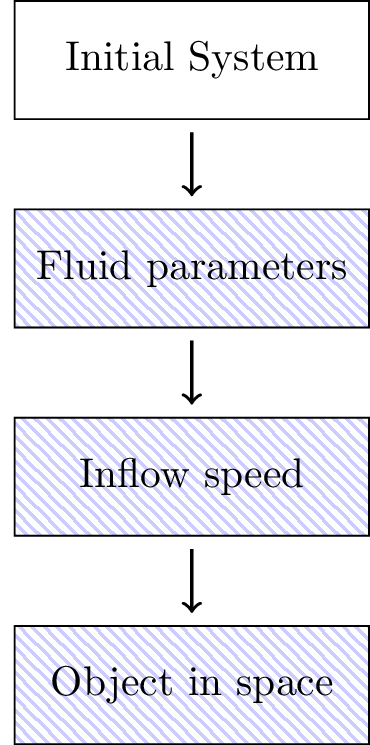
\includegraphics[scale=0.25]{images/meth/meth_7}
    \end{column}
    \begin{column}[c]{0.65\textwidth}
      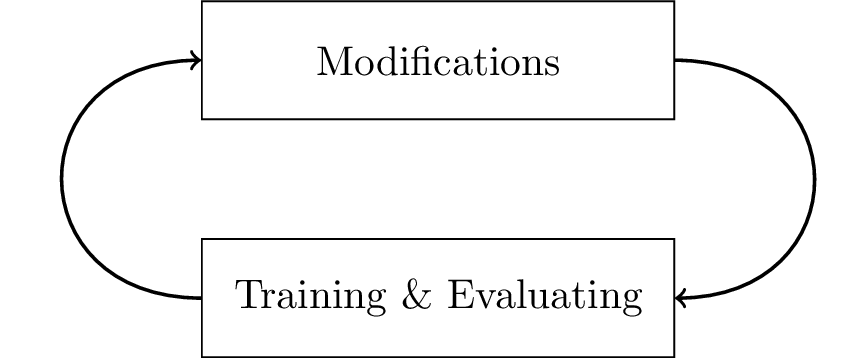
\includegraphics[scale=0.22]{images/meth/mod_train}
    \end{column}
  \end{columns}
\end{frame}



\section{Development}

\begin{frame}[t]
  \frametitle{Project Development}
\end{frame}


\begin{frame}[t]
  \frametitle{Project Development}
  \large{\textbf{Data Generation}}
\end{frame}



\begin{frame}[t]
  \frametitle{Project Development}
  \large{\textbf{Data Generation}}

  \begin{itemize}
  \item The simulation has several adjustable parameters
    \begin{itemize}
    \item inflow speed
    \item fluid viscosity
    \item fluid density
    \end{itemize}
  \end{itemize}
  
\end{frame}

\begin{frame}[t]
  \frametitle{Project Development}
  \large{\textbf{Data Generation}}
  \begin{itemize}
  \item The simulation has several adjustable parameters
    \begin{itemize}
    \item What is a good choice for the parameters.
    \end{itemize}
  \end{itemize}
\end{frame}


\begin{frame}[t]
  \frametitle{Project Development}
  \large{\textbf{Data Generation}}
  \begin{itemize}
  \item The simulation has several adjustable parameters
    \begin{itemize}
    \item Reynold's number in the range of [90, 350]
    \end{itemize}
  \end{itemize}
\end{frame}

\begin{frame}[t]
  \frametitle{Project Development}
  \large{\textbf{Data Generation}}
  \begin{itemize}
  \item The simulation has several adjustable parameters
    \begin{itemize}
    \item Reynold's number in the range of [90, 350]
    \end{itemize}
  \end{itemize}
  \begin{center}
    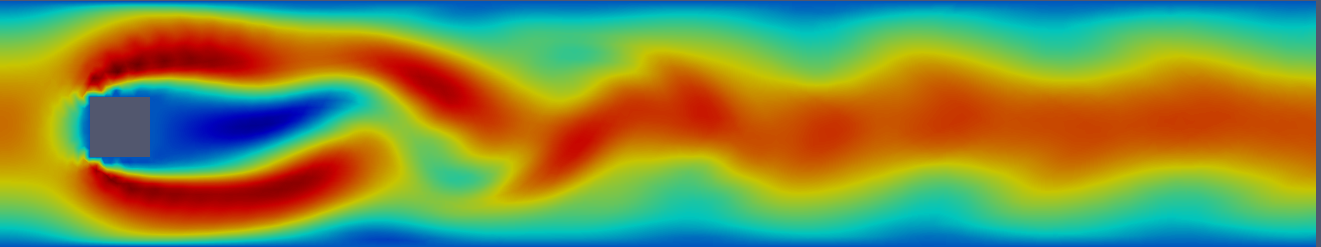
\includegraphics[scale=0.21]{images/x-direction}
  \end{center}
  \begin{center}
    \begin{figure}[htb]
    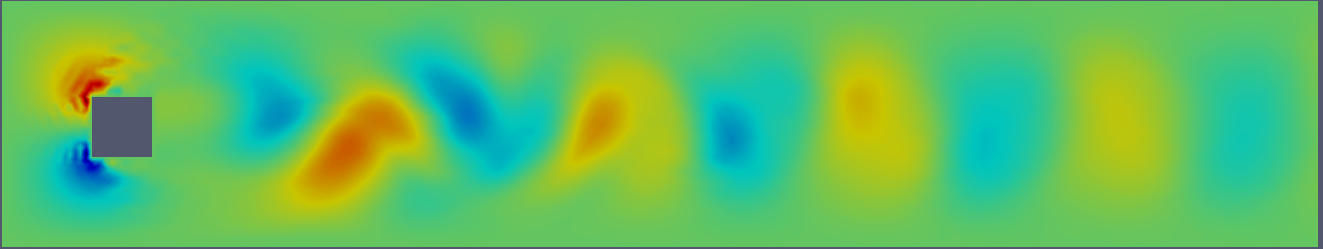
\includegraphics[scale=0.21]{images/y-direction} \\
    \caption{Karman vortex street}
    \end{figure}
  \end{center}
\end{frame}


\begin{frame}[t]
  \frametitle{Project Development}
  \large{\textbf{Data Generation}}
  \begin{itemize}
  \item Choosing appropriate color space
    \begin{itemize}
    \item Grayscale
    \item RGB
    \end{itemize}
  \end{itemize}  
  \begin{center}
    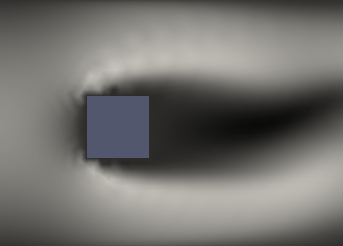
\includegraphics[scale=0.27]{images/x-direction-gray} \hspace{0.7cm}
    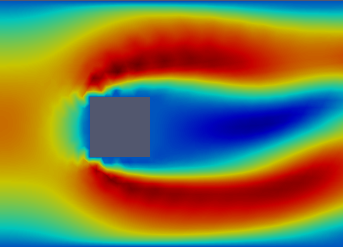
\includegraphics[scale=0.27]{images/x-direction-rgb} \\ \vspace{0.2cm}
    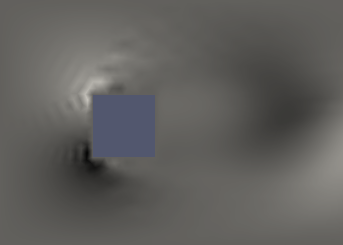
\includegraphics[scale=0.27]{images/y-direction-gray} \hspace{0.7cm}
    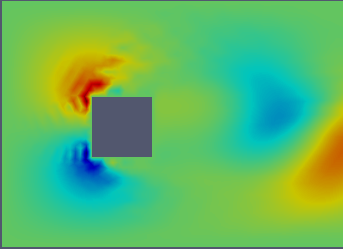
\includegraphics[scale=0.27]{images/y-direction-rgb} \\
  \end{center}  
\end{frame}


\begin{frame}[t]
  \frametitle{Project Development}
  \large{\textbf{Models}}
\end{frame}

\begin{frame}[t]
  \frametitle{Project Development}
  \large{\textbf{Models}}
  \begin{itemize}
  \item Two types of architectures based on our preliminary research:
  \end{itemize}
\end{frame}

\begin{frame}[t]
  \frametitle{Project Development}
  \large{\textbf{Models}}
  \begin{itemize}
  \item Two types of architectures based on our preliminary research:
    \begin{itemize}
    \item ResNet 
    \end{itemize}
  \end{itemize}
  \vspace{1cm}
  \begin{center}
      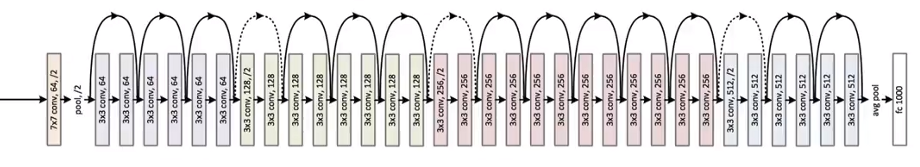
\includegraphics[scale=0.37]{images/nets/res}
    \end{center}
\end{frame}


\begin{frame}[t]
  \frametitle{Project Development}
  \large{\textbf{Models}}
  \begin{itemize}
  \item Two types of architectures based on our preliminary research:
    \begin{itemize}
    \item UNet
    \end{itemize}
  \end{itemize}
  \vspace{1cm}
  \begin{center}
    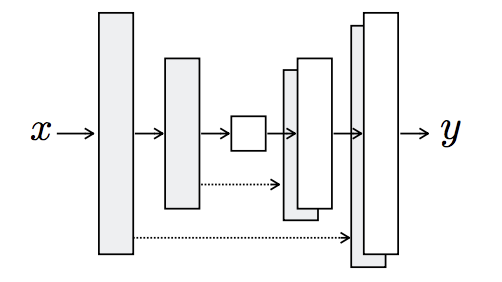
\includegraphics[scale=0.37]{images/nets/unet}
  \end{center}  
\end{frame}


\begin{frame}[t]
  \frametitle{Project Development}
  \large{\textbf{Data Use}}
\end{frame}


\begin{frame}[t]
  \frametitle{Project Development}
  \large{\textbf{Data Use}}
  \begin{itemize}
  \item Usage of pressure field
  \end{itemize}
  \vspace{0.5cm}
  \begin{center}
    \includegraphics[scale=0.20]{images/models/pressure_optional}
  \end{center}  
\end{frame}


\begin{frame}[t]
  \frametitle{Project Development}
  \large{\textbf{Data Use}}
  \begin{itemize}
  \item Usage of pressure field $\rightarrow$ the pressure field turned out to be useful
  \end{itemize}
  \vspace{0.5cm}
  \begin{center}
    \includegraphics[scale=0.20]{images/models/pressure_optional}
  \end{center}  
\end{frame}



\begin{frame}[t]
  \frametitle{Project Development}
  \large{\textbf{Data Use}}
  \begin{itemize}
    \item Processing of real values
  \end{itemize}
  \vspace{0.5cm}
  \begin{center}
    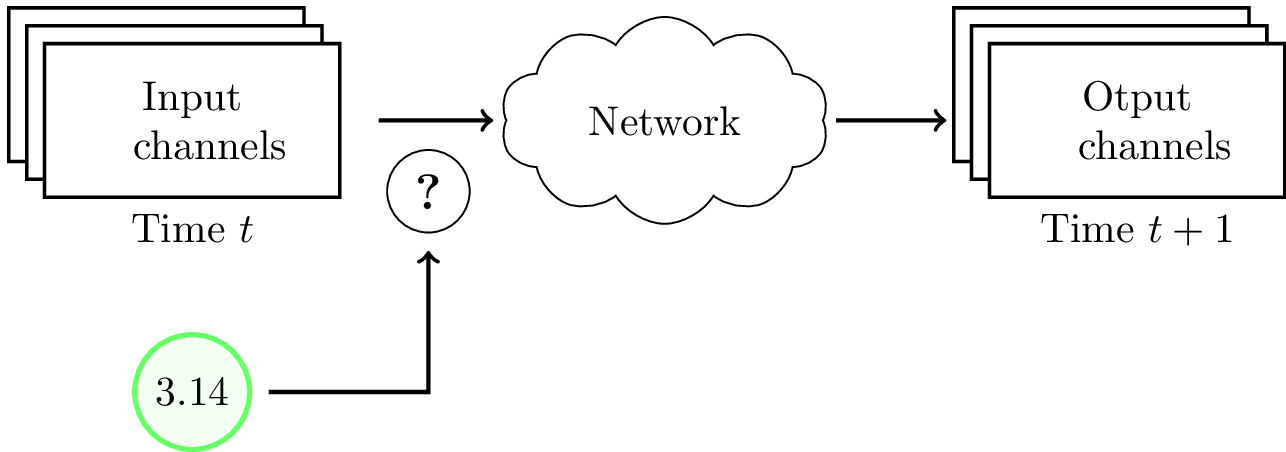
\includegraphics[scale=0.20]{images/models/num_question}
  \end{center}  
\end{frame}

\begin{frame}[t]
  \frametitle{Project Development}
  \large{\textbf{Data Use}}
  \begin{itemize}
    \item Processing of real values $\rightarrow$ extra image channel filled with the value
  \end{itemize}
  \vspace{0.5cm}
  \begin{center}
    \includegraphics[scale=0.20]{images/models/num_answer}
  \end{center}  
\end{frame}

\begin{frame}[t]
  \frametitle{Project Development}
  \large{\textbf{Results consideration}}
  \vspace{-0.5cm}
  \begin{columns}[t]
    \begin{column}{0.5\textwidth}
      \begin{center}
        {\large \underline{Image processing}}
      \end{center}
    \end{column}
    \begin{column}{0.5\textwidth}
      \begin{center}
        {\large \underline{Numerical Simulation}}
      \end{center}  
    \end{column}
  \end{columns}  
\end{frame}



\begin{frame}[t]
  \frametitle{Project Development}
  \large{\textbf{Results consideration}}
  \vspace{-0.5cm}
  \begin{columns}[t]
    \begin{column}{0.5\textwidth}
      \begin{center}
        {\large \underline{Image processing}}
        \begin{itemize}
        \item Perceived qualities of the \underline{image} results
        \item Metrics:
          \begin{itemize}
          \item Peak signal-to-noise ratio - PSNR
          \item Correlation
          \end{itemize}
        \end{itemize}
      \end{center}
    \end{column}
    \begin{column}{0.5\textwidth}
      \begin{center}
        {\large \underline{Numerical Simulation}}
      \end{center}  
    \end{column}
  \end{columns}
\end{frame}


\begin{frame}[t]
  \frametitle{Project Development}
  \large{\textbf{Results consideration}}
  \vspace{-0.5cm}
  \begin{columns}[t]
    \begin{column}{0.5\textwidth}
      \begin{center}
        {\large \underline{Image processing}}
        \begin{itemize}
        \item Perceived qualities of the \underline{image} results
        \item Metrics:
          \begin{itemize}
          \item Peak signal-to-noise ratio - PSNR
          \item Correlation
          \end{itemize}
        \end{itemize}
      \end{center}
    \end{column}
    \begin{column}{0.5\textwidth}
      \begin{center}
        {\large \underline{Numerical Simulation}}
        \begin{itemize}
        \item \underline{Real} differences between the predicted and the actual \underline{values}
        \item Metrics:
          \begin{itemize}
            \item Average percentage difference
            \item Max percentage difference
          \end{itemize}
        \end{itemize}
      \end{center}  
    \end{column}
  \end{columns}
\end{frame}


\begin{frame}[t]
  \frametitle{Results}
  % Images of individual images
\end{frame}

\begin{frame}[t]
  \frametitle{Results}
  % Images of timestep
\end{frame}

\begin{frame}[t]
  \frametitle{Results}
  % Images of recursive application
\end{frame}

\begin{frame}[t]
  \frametitle{Results}
  % Raw results but much less than before
\end{frame}


\begin{frame}[t]
  \frametitle{Results}
  % Numbrs of the recursive application
\end{frame}


\begin{frame}[t]
  \frametitle{Further development}
  % time checks
  % Difference images
  % Using the mask for the object
\end{frame}







  

% \section{Timeplan}
% \begin{frame}[t]
%   \frametitle{Timeplan}
%   \begin{center}
%     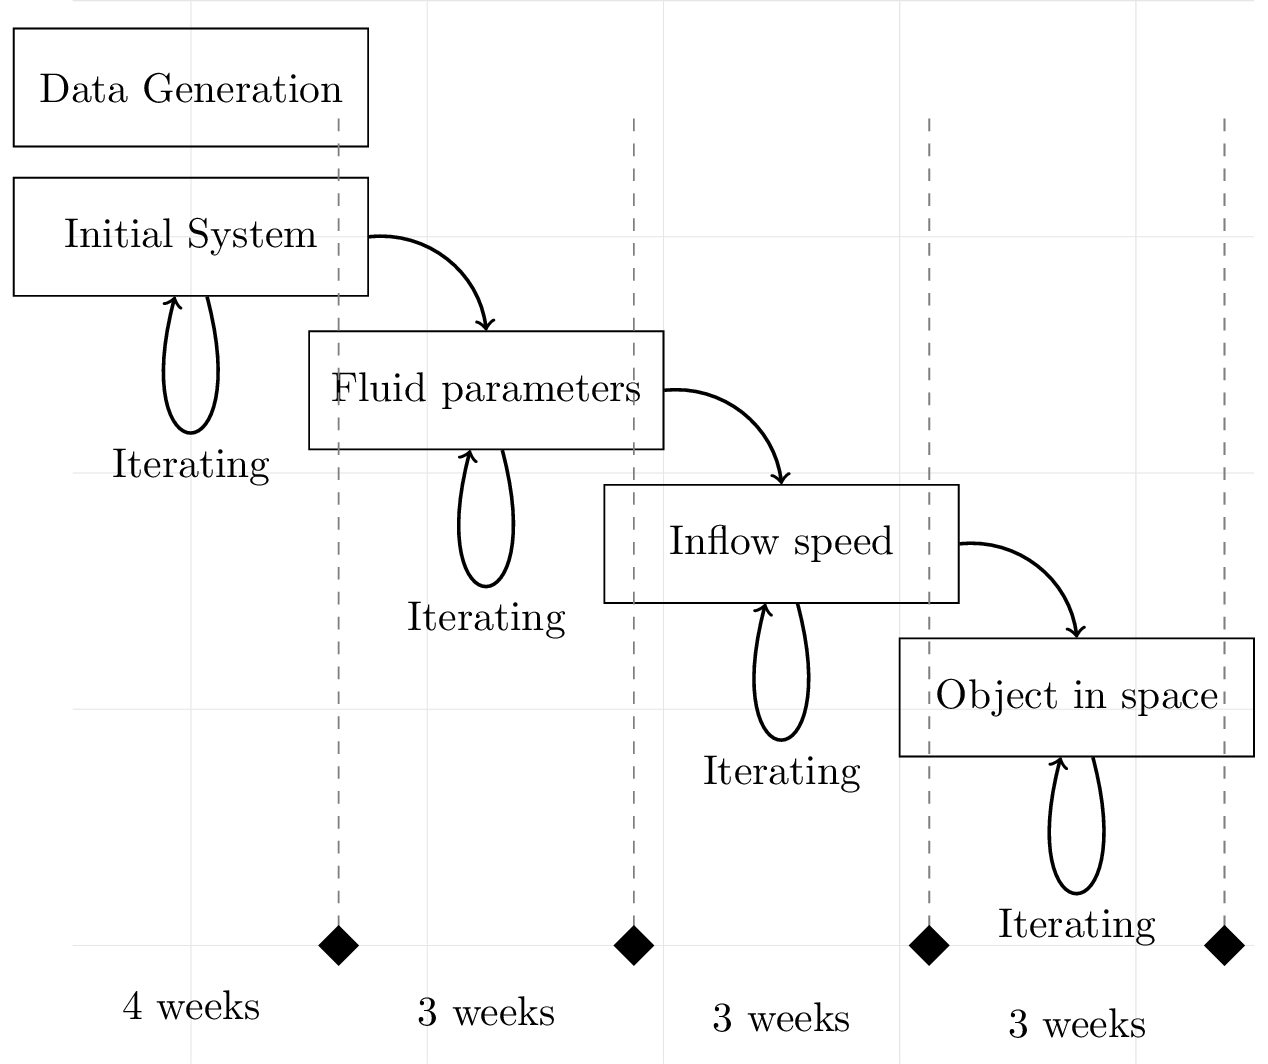
\includegraphics[scale=0.19]{images/time}
%   \end{center}
% \end{frame}


\section{Conclusion}

\begin{frame}
  \frametitle{}
  \begin{center}
    \huge{Thank you for your attention.}
  \end{center}
\end{frame}

\begin{frame}
  \frametitle{}
  \begin{center}
    \huge{Questions?}
  \end{center}
\end{frame}

\end{document}

% LocalWords:  incompressible

%%% Local Variables:
%%% mode: latex
%%% TeX-master: t
%%% End:
